\documentclass[output=paper]{LSP/langsci} 
\ChapterDOI{10.5281/zenodo.1090974}
\title{News Translation: Text analysis, fieldwork, survey}
\author{Rovena Troqe\affiliation{University of the Free State, South Africa \newline University of Geneva, Switzerland \newline Fonds National Suisse de la recherche scientifique (FNS) \newline Centre de Recherches Sémiotiques (CeReS)}\lastand Francis Marchan\affiliation{Groupe de Recherches et d'Etudes Sociologiques du Centre Ouest (GRESCO)}}

\abstract{In this study, we investigate the practice of news translation in order to examine the participation of actants who play a role in the production of a translation and who contribute to defining what translation is or should be. The conceptual framework applied in the study combines the generative semiotic theory and a hybrid methodological approach based on semiotic discourse analyses with textual corpora, think-aloud protocols with news editors and a survey among the readers of the translated texts. This triangulation of data sheds light on the publishing workflow and on the reception of translations, and helps understand how the various ways in which different actants conceptualize translation come together, which one prevails and on what grounds.}

% Are these to be included?
%\textbf{Key-words:} news translation, semiotic discourse analysis, think aloud protocol, survey among reader of translations

\begin{document}
\maketitle

\section{Background: Translating news}

Translation studies scholars have shown that translation is a crucial factor in disseminating news in the (inter)national arena. Researchers have focused on news agencies and have mapped local and global networks of journalists in order to understand how news is gathered and distributed and how translation is performed by and for news agencies \citep{Bielsa2007, Bielsa2009}. The norms and style of the journalistic genre have been investigated in order to identify how the original text is restructured, shaped, transformed or even merged with other news sources into a different target text that better suits a different linguistic, cultural and geographical context \citep{Stetting1989, Bielsa2007, Tapia1992, Bielsa2007, Brownlie2010, Caimotto2010, Tsai2010, Federici2010, Gumul2010}. Case studies show that when translation is integrated into journalism, it is governed by norms that fall into the category of news production, that it is performed by trained and specialized journalists who are not translators and usually remain invisible (\citealt{Tapia1992, Bielsa2007, Bielsa2009, Schaffner2010}: \citealt{Hernandez2011}) and eventually that concepts such as equivalence and faithfulness are of minor importance compared to journalistic norms, medium constraints and adjustments to the target audience \citep{Stetting1989, Pym2004, Bielsa2009}. 

With the study of news translation practices, scholars have raised questions as to who decides what news is published in newspapers and how news is translated and approved before publishing, which techniques are adopted so as to better fulfill media goals, and how all of this affects the modern theory and practice of translation. From a methodological perspective, these contributions are mostly, though not exclusively, based on text analysis, as they apply critical and political discourse analysis. Some field research is also carried out in order to investigate daily work in news agencies \citep{Bielsa2009, Tsai2010} or via face-to-face interviews \citep{Brook2012}. 

This study tries to address some of the above questions by investigating a specific practice of news translation, in the \ili{Italian} magazine Internazionale, using a new conceptual framework --  generative semiotic theory -- and a hybrid qualitative methodological approach, i.e. by combining semiotic discourse analysis with textual corpora, think-aloud protocols with the editors of Internazionale and a survey among the magazine's readership. The idea here being that by using different types of analyses the results become more rigorous and the phenomenon will be more fully understood. In fact, authors from other disciplines have stressed the importance of methodological \isi{triangulation}, helping to strengthen the trustworthiness of the findings. Triangulation consists in the use of multiple data sources by multiple researchers espousing multiple theoretical perspectives and methods \citep{Leech2007, Jensen2008Credibility}. 

The main goal is to describe as accurately as possible, and with the use of different sources of data and data gathering techniques, the voices of the actants who play a role in the practice of translation and contribute to defining what translation is or should be. 

The sociological turn in translation has shed light on the study of the multiple actors involved in the production of translations. Some authors adopt a Bourdieusian approach to translation, where it is seen as an artistic product with a symbolic capital \citep{Inghilleri2005, Gouanvic2005, Gouanvic2007}; other authors bypass purely textual approaches to translation in order to understand how the circulation of texts depends on power relations between agents that participate in the practice \citep{Heilbron2002, Heilbron2007, Sapiro2008}; others apply Latour's actor-network theory to identify and describe the role of actors participating in the generation and circulation of translations \citep{Buzelin2005, Buzelin2006,Buzelin2007a,Buzelin2007b, Bogic2010}. Most of these studies are based on qualitative methods combining fieldwork, interviews and observations with the analysis of written documents.

Although social studies have focused mainly on the book industry and on literary translation (little attention has been devoted to the translation of other text typologies), the sociological approach has the great merit of having unveiled the presence of hidden actors taking part in the \isi{translation process}, thus contributing to defining -- or blurring-- the boundaries of translation. 

In consonance with recent studies in the field of news translation, and acknowledging the need to understand translation practices in a broader way, this study adopts a semiotic approach that makes it possible to:

\begin{itemize}
 \item identify shifts in translated and edited texts containing voices of different subjects that transform these texts;
 \item identify these voices as \textit{actants} that operate in manipulative, performative and sanctioning modalities, according to specific systems of values.
\end{itemize}


\section{Conceptual framework: The semiotic perspective}

A semiotic model of the practice of translation and a semiotic definition of the concept of translation are adopted here as a conceptual framework.

As stated in \citet{Troqe2014a, Troqe2014b}, the semiotic\footnote{Here we are referring to Greimassian semiotics \citep{Greimas1970, Greimas1983, Greimas1979, Fontanille2003}} concept of \textit{narrativity} is considered to be the organizing principle of discourses, including scientific discourse. Narrativity allows for a description of translation as the result of the manipulation, performance and sanction by two main actants:\footnote{In the semiotic perspective, an actant accomplishes or undergoes qualifying acts. An actant may be an individual or a group of individuals.}  the Initiator and the Translator. In the semiotic perspective, the action of somebody doing something is called \textit{Manipulation}\footnote{According to Jeremy Munday, in Translation Studies, the concept of ideology has a negative connotation involving distortion, concealment and manipulation; thus, translation is seen as manipulative distortion and rewriting \citep[196]{Munday2007}. By adopting a Semiotic perspective, we consider any act of Manipulation as a triggering act of translation, performed by an actant called Initiator on an actant called Translator. This outlook allows for a neutral stance on manipulation and sees it as a prerogative of the Initiator.}. In our approach, Manipulation, in Translation, qualifies the actant Initiator, who acts on another actant, the Translator, for him/her to carry out a given translational programme. The Translator actant may or may not adhere to specific programmes of translation. Manipulation and adherence set the stage for a contractual situation where translational requirements are to be fulfilled by the Translator. These requirements influence the performance of the Translator and the result of his/her action. Sanction follows performance: the Initiator assesses the compatibility of the performance with the contractual requirements and with his/her system of values by accepting, \isi{revising}, amending, adapting, altering, reshaping and aligning the translated text with a specific system of values. The investigation of interactions between the Initiator and the Translator is performed by another actant, the Researcher, whose stance, beyond any claim of objectivity, must be included in the semiotic model that is presented here (\figref{troqe-marchan:fig:1}).

%% we don't need this:
% \begin{tabularx}{\textwidth}{X}
% \lsptoprule
% 
%  \rmfamily\bfseries Semiotic Model of Translation \\
% \rmfamily \textbf{Researcher} \\
% \begin{tabularx}{\textwidth}{XX}
% \lsptoprule
% 
% \multicolumn{2}{X}{ \rmfamily\bfseries Translation Programme}\\
% \rmfamily Initiator & \rmfamily Translator\\
%  {\rmfamily %
% %but manipulation can also be due to the translator {}- shouldn't it be placed somewhere in the middle between both actants? See footnote 3
% Manipulation}\par
% 
%  {\rmfamily persuasion, prescription}\par
% 
%  {\rmfamily} \par
% 
%  {\rmfamily \textbf{\textit{Contractual}}\textbf{ }\textbf{\textit{instructions}}}\par
% 
%  \rmfamily \textbf{\textit{System of values} }
%  \rmfamily Sanction & {\rmfamily Competence}\par
% 
%  {\rmfamily acceptance/resistance}\par
% 
%  {\rmfamily [Warning: Draw object ignored]}\par
% 
%  {\rmfamily Performance}\par\\
% \lspbottomrule
% \end{tabularx}
% {\rmfamily  \textbf{Epistemic act on:}}
% 
% {\rmfamily\bfseries\itshape Ethical and normative dimension} 
% 
% \rmfamily \textbf{\textit{Enunciative praxis and textual dimension} }\\
% \lspbottomrule
% \end{tabularx}

\begin{figure}
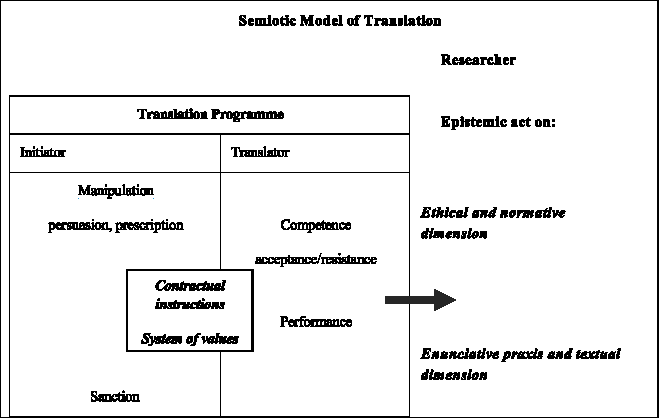
\includegraphics[width=\textwidth]{figures/troqe-marchan/figure1.pdf}
\caption{Semiotic model of translation}
\label{troqe-marchan:fig:1}
\end{figure}

\largerpage
Regardless of what the translational practice is, what steps the actants may take and what the specific translation requirements are, from a semiotic perspective, two concepts must be considered inherent to any practice or idea of translation: \textit{equivalence} and \textit{difference}. \textit{Difference} refers to the concept of contrast: in order for it to be and emerge as an individual and unique entity, the Translation must first be different from the thing to which it refers -- the Original, the other. Translation is a different subject, a different linguistic expression, a different practice. The term \textit{equivalence} refers to a condition of derivation, to the need for the Translation to emerge as a reference, an analogy, a simulation or a copy of something else (the Original)\footnote{The concept of \textit{equivalence} is an immanent feature in the theoretical discourse on translation and translating; implicitly or explicitly, and regardless of how it has been defined, the term \textit{equivalence} has influenced and regulated the practice and theory of translation over time, becoming a supermeme \citep{Chesterman1997} and an immanent condition to translation. However, recent developments in the field underline the paradoxical condition that characterises the concept of translation. The undeniable non-equivalence of translation compared to the original, whether conceptual, ontological, pragmatic, semantic, in the medium, in the finality and so on, is evident, and the idea of \textit{difference} is clearly theorised by translation scholars: In particular, the ``similar but different'' concept in \citet{Nida2004}, ``divergent similarity'' in \citet{Chesterman1996} but also in the semiotic writings of \citet{Stecconi2004, Gorlee1994, Petrilli1992}, translation is seen as a purposeful equivalent but different activity.}. In this perspective and as formulated, in a similar way, by Gideon Toury, \textit{equivalence} entails a certain interference of the underlying source structure -- in terms of linguistic and textual conventions and decision not to adapt the translation to the target system requirements, while on the other hand, \textit{difference} yields ``subjugation'' to the recipient system, involves suppression of source specific features, or even recreation or addition of new features in order to enhance \isi{acceptability} in the target system \citep[171]{Toury1995}.

The question of confrontation of identities (I \textit{vs.} Other) represents a third inherent aspect in the study of translation. It refers to the derivation, exchange, resistance, compatibility or incompatibility between the Translation-I -- the translating identity -- and the Original-Other. 

Those terms are adopted in the Greimassian semiotic square\footnote{As an elementary structure of meaning, the semiotic square defines the fundamental conditions of existence of a concept, an individual or society (\citealt{GreimasRastier1968}, 87).} to formalize the translation paradox -- the simultaneity of equivalence and difference and the confrontation of the identity Translation-I vs. Original-Other (\figref{troqe-marchan:fig:2}).

%% we don't need this
% \begin{tabularx}{\textwidth}{X}
% \lsptoprule
% {\rmfamily [Warning: Draw object ignored]}
% 
% {\rmfamily \textbf{%
% %please use consistent notation
% Translation /}\textbf{I}}
% 
% {\rmfamily [Warning: Draw object ignored][Warning: Draw object ignored][Warning: Draw object ignored][Warning: Draw object ignored][Warning: Draw object ignored][Warning: Draw object ignored][Warning: Draw object ignored]difference  equivalence}
% 
% {\rmfamily [Warning: Draw object ignored][Warning: Draw object ignored]\textbf{alterity  similarity}}
% 
% {\rmfamily non-equivalence  non-difference}
% 
% \rmfamily\bfseries Other / Original\\
% \lspbottomrule
% \end{tabularx}

\begin{figure}
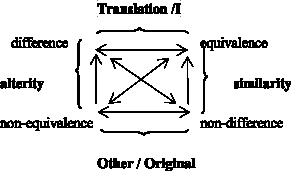
\includegraphics[width=.5\textwidth]{figures/troqe-marchan/figure2.pdf}
\caption{Semiotic square of translation} 
\label{troqe-marchan:fig:2}
\end{figure}

The semiotic square of Translation depicts virtual and abstract values that emerge from different translation practices by different actants, who operate in different contexts and cultures. 
\newpage 

The conceptual framework -- the semiotic model and the semiotic square of translation -- is adopted here to investigate the translation practice of written news published by the \ili{Italian} magazine Internazionale. 

Theoretical reasoning is backed up by empirical research designed to gather data from: 

\begin{itemize}
 \item the analysis of a sample of original, translated and edited texts published by Internazionale with the label translation;
 \item verbalisations by four Internazionale editors while working on translated texts and thinking aloud;
 \item a survey among readers of Internazionale who expressed their opinion on translation in general and on translation by Internazionale in particular. 
\end{itemize}


\section{Results and discussion}

\subsection{Text analysis}\label{troqe-marchan:sec:a} % former section a)

Internazionale is an \ili{Italian} weekly magazine founded in 1993 that publishes %
%from which \isi{source language}(s)
translated articles (from all languages from Asian to African languages, but mainly from European languages) from the international press, the main goals being to inform and provide the readers with a more nuanced and richer perspective compared to other \ili{Italian} periodicals. According to one of the four deputy directors\footnote{Interview of 28\textsuperscript{th} June, 2013 with a deputy director of Internazionale.}  of the magazine, three main criteria are of importance in selecting articles worthy of being published in Internazionale: respect for journalistic standards (clarity and accuracy in facts and style); impact and appeal; variety of sources. Another important criterion is the feasibility of shortening texts: usually articles are only chosen if it is possible to carry out editorial cuts without ``changing the meaning''. 

The publishing workflow consists of different phases: 

\begin{itemize}
 \item Original texts are usually selected and often treated (i.e. shortened) by in-house editors. Each editor is a specialist for specific geographical areas and topics.
 \item Selected texts are discussed and chosen at the weekly editorial board meeting. The number of pages in the magazine to be assigned to each text is also discussed.
 \item Texts are sent to freelance professional translators with deadlines ranging from 24 hours to a week.
 \item Translations are edited by the editors and reviewed by the copy editors and the director general before publishing. Revision by the copy editors is only done on the edited texts and is mostly aimed at coherence of content, consistency and accuracy in the \ili{Italian} language. 
\end{itemize}


The first part of this study focused on 28 articles published by the magazine in the period 2011--2012. A semiotic analysis was performed on the translations (from English, \ili{French} and \ili{German}) and edited translations. Comparisons with the originals allowed major cuts and other types of shifts to be identified. %
%reference?
QDA Miner qualitative data analysis software\footnote{http://provalisresearch.com/products/qualitative-data-analysis-software/} was used to annotate texts manually and extract information from the corpora. 

An initial exploration of the textual data gives us an overview (\figref{troqe-marchan:fig:3}) of the percentage of words in the original, translated and edited texts. Regarding the total number of words in the original texts (35'596 words in total), there were 2.2\% fewer words in the translated texts (34'837 words in total) and roughly 22\% fewer words in the published articles (27'908 words in total).\footnote{These figures aggregate the English results (89.79\% of words in the translated texts and 77.07\% in the published articles compared to the originals), the \ili{French} results (98.23\% of words in the translated texts and 73.93\% in the published articles compared to the originals) and the \ili{German} results (118.79\% of words in the translated texts and 84.79\% in the published articles compared to the originals).}


\begin{figure}
	\begin{tikzpicture}
        \begin{axis}[
            width  = .8\textwidth,
            height = .3\textwidth,
            ylabel={\%},
            xlabel={}, 
            symbolic x coords={Originals (35'596), Translation (34'837), Internazionale (27'908)},
            xtick=data,
            axis lines*=left,  
            ymin=0,
            ybar,
            bar width = 36pt,
            nodes near coords,
            nodes near coords align={vertical},
            axis on top,
            ymajorgrids, tick align=inside,
            major grid style={draw=white},
            enlarge x limits=true, 
       	]    
        \addplot+[blue!80!black,fill=lsMidBlue] coordinates {(Originals (35'596),100) (Translation (34'837),97.80) (Internazionale (27'908),78.04)};
        \end{axis}
    \end{tikzpicture}
%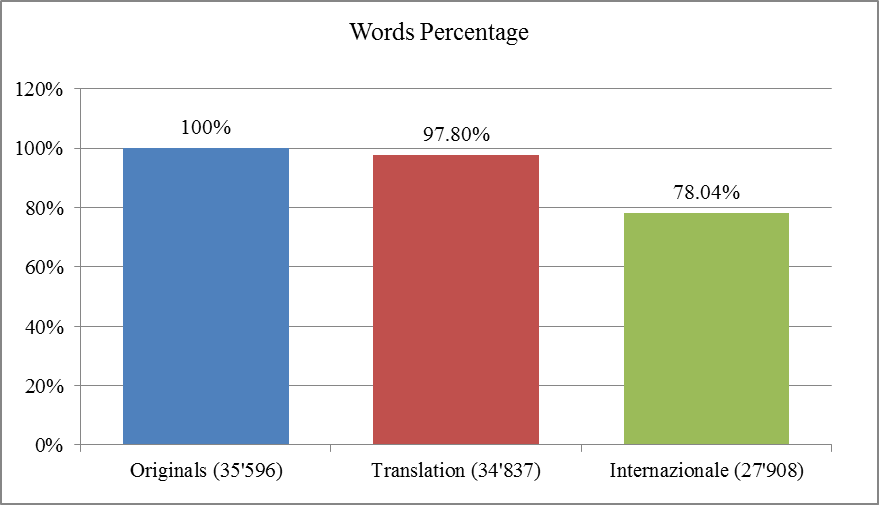
\includegraphics[width=\textwidth]{figures/troqe-marchan/figure3.png}
\caption{Average words in translations and originals}
\label{troqe-marchan:fig:3}
\end{figure}

For a detailed analysis, semiotic categories \citep[200--202]{Fontanille2006, Fontanille1998} were used to identify variations in the translated texts and published articles. Below is a description and a few examples of the semiotic categories used to annotate shifts in the textual corpora.

\subsubsection{Omission}

Disappearance of forms and dilution in virtual structures -- the elimination of expressions, sentences and paragraphs in the target texts. 

%\todo{Table not referenced}
%\todo{check all references to tables}
%\todo{maybe more expressive table captions?}
\begin{sidewaystable} 
 \scriptsize
 \caption{Omission}
 \label{troqe-marchan:tab:1}
\begin{tabularx}{\textwidth}{Q  p{5cm} p{3cm}}
\lsptoprule
 Original &  Translation & Internazionale \\
 \midrule
 (\ldots ) A spokesperson for MINUSTAH did not respond to e-mailed questions, but the United Nations has denied that soldiers were sick.

 Waldor says he finds Piarroux's evidence ``suggestive but not absolutely conclusive.'' There are ways to collect more evidence -- for instance, by testing the Nepalese soldiers for antibodies against \textit{V. cholerae}. ``It may be getting late for that,'' Waldor cautions, because antibodies peak after about a month.

 Some scientists don't believe foreigners introduced cholera at all, despite the molecular clues. Most prominent among them is Rita Colwell, a veteran microbiologist at the University of Maryland, College Park. Colwell believes that most cholera outbreaks are caused by bacteria that lurk locally and proliferate when conditions are favourable -- in this case, perhaps a climate event called La Niña. To Waldor, the idea that a microbe so closely resembling a South Asian strain would emerge in Haitian waters is ``frankly absurd.'' \textit{(Colwell e-mailed} Science \textit{that she was ``in Bangladesh working on cholera and unable to respond'' to questions.)}

{\itshape If the Nepalese introduced cholera, says Waldor, several measures could be considered to prevent a repeat. Aid workers or peacekeepers from cholera-endemic countries who are sent to cholera-free but vulnerable places like Haiti could be screened in advance, for instance, or given prophylactic antibiotics.
But Harvard cholera scientist Edward Ryan counters that testing thousands of soldiers using rectal swabs would be time-consuming and costly--and that testing isn't very accurate. Prescribing antibiotics would pose problems, such as adverse reactions and cause drug resistance in V. cholerae and other microbes. What's more, says CDC epidemiologist Eric Mintz, businesspeople, visiting relatives, and tourists would also have to be tested. ``It wouldn't be very practical,'' Mintz says.}

 ``Despite Sensitivities, Scientists Seek To Solve Haiti's Cholera Riddle'', Science, Science 331 (6016), 388-389, January 28, 2011 &
 
\raggedright 
 (\ldots ) ''Un portavoce della Minustah non ha risposto alle domande inviate per email, ma le Nazioni Unite hanno negato che i soldati fossero malati.

{\itshape Per Waldor le prove di Piarroux sono ``indicative ma non definitive''. Esistono modi di scovarne altre, per esempio testando i soldati nepalesi alla ricerca di anticorpi contro il vibrione del colera. ``Tuttavia potrebbe essere troppo tardi'', avverte Waldor, perché gli anticorpi raggiungono il picco massimo dopo circa un mese.
Malgrado gli indizi molecolari, alcuni scienziati non credono affatto che siano stati gli stranieri a portare il colera. La più importante tra loro è Rita Colwell, un'esperta microbiologa della University of Maryland, a College Park, convinta che la maggior parte delle epidemie di colera sia causata da batteri che si annidano sul posto e proliferano in condizioni favorevoli, in questo caso forse per l'evento climatico chiamato La Niña. Per Waldor l'ipotesi che un microbo così simile al ceppo dell'Asia meridionale possa emergere nelle acque haitiane è ``francamente assurda''.} & 

{\raggedright
Un portavoce della Minustah non ha risposto alle domande di Science inviate per email, ma le Nazioni Unite hanno negato
che i soldati fossero malati.} \\
\\
\lspbottomrule
\end{tabularx}
\end{sidewaystable}

\subsubsection{Revolution}

Major variations that radically change the meaning of the original text. Revolutions may occur concomitantly with other types of variations, e.g. original contents are omitted and replaced by new sentences that cause shifts in the argumentative positions. \tabref{troqe-marchan:tab:2} provides an excerpt from the article ``The Chemistry of the Suppression of Desire: What is going on in the brain of a cheater?'' published by Slate Magazine and translated into \ili{Italian} by Internazionale. The translated version appears in the second column; it is common practice for the original texts to be ``edited'', i.e. shortened, before being sent to the translator, in fact, in  \tabref{troqe-marchan:tab:3}, the central paragraph (``But there's a problem [\ldots]  to satisfy fleeting desire'') is missing in the translated version. An illustration of the ``revolution'' variation can be found in the last paragraph in \tabref{troqe-marchan:tab:2}, which encapsulates the take-home message. It is transformed in the edited version as follows ``In spite of the genetics, we are responsible for our actions'', a sentence that contradicts the argumentative stance of the original, which aims at maintaining a rather nuanced stance towards infidelity and evaluating the role that genetics plays in human behaviour. 

\begin{table}
 % TODO
 \tiny
 \caption{Revolution}
 \label{troqe-marchan:tab:2}
\begin{tabularx}{\textwidth}{p{5cm}XX}
\lsptoprule
 Original & Translation & Internazionale \\
 \midrule{}
 [\textit{Larry believes that kissing}], hugging, caressing, and intimate small talk can all help to keep a man's oxytocin high, too

{\itshape [But there's a problem with this takeaway message. The longer we're with our social partner, the less intimacy and sex we have. When new mates are first introduced, they have sex like crazy. After a time--in marmosets, for example, it's about 80 days--they won't be having much sex at all.
Less sex does not mean we're less devoted. We have other powerful reasons to maintain the social relationship, not least CRF. But depending at least partly on our genetic makeup, our motivation to seek erotic reward can be more or less powerfully awakened by a new potential partner. If the circuit shouts loudly enough, we'll risk the committed relationship, our careers, and our reputations to satisfy fleeting desire.]}

We're not automatons. We are responsible for our actions. But our baked-in biases can make us susceptible to infidelity. Our brains can be a battlefield of competing interests, and sometimes desire wins. It may win more often in people like Petraeus whose bold, creative thinking we so admire can come with a bias toward behavior we don't. That doesn't make him special, it makes him human.

The Chemistry of the Suppression of Desire What is going on in the brain of a cheater?, Slate, 27.12. 2012 & 
[\ldots] Ed è anche possibile che baci, abbracci, carezze e confidenze intime servano a mantenerla alta. [\ldots]

Ad ogni modo non siamo automi. Siamo responsabili delle nostre azioni, eppure le inclinazioni ormai radicate rischiano di renderci infedeli. Il nostro cervello può essere un terreno di scontro tra interessi conflittuali e a volte vince il desiderio. Forse vince più spesso in quelli come Petraeus, il cui modo di pensare audace e creativo che tanto ammiriamo può essere accompagnato dalla propensione a un comportamento che invece non apprezziamo. & 
Malgrado la genetica, siamo responsabili delle nostre azioni. \\
\lspbottomrule
\end{tabularx}
\end{table}

\subsubsection{Emergence}
\largerpage
\begin{table}[b]
 \tiny
 \caption{Emergence}
 \label{troqe-marchan:tab:3}
\begin{tabularx}{\textwidth}{XXX}
\lsptoprule
 Original &  Translation &  Internazionale \\
 \midrule
Einzelne Schwellenländer sind dafür, da sie indirekt bereits mit den Folgen der europäischen Krise kämpfen; ihre Währungen werden wegen des Rückzugs aus Euroanlagen nämlich immer stärker. 

 G-20 erhöhen Druck auf Europa, Der Standard, 16.11.2011 &  Alcuni paesi emergenti sarebbero favorevoli, in quanto già si stanno confrontando indirettamente con le conseguenze della crisi europea: a causa della rinuncia agli investimenti in Europa, le loro valute si stanno infatti rafforzando progressivamente.  & Alcuni paesi emergenti sarebbero favorevoli, perché già subiscono le conseguenze della crisi europea\textbf{: molti investitori hanno deciso di portare via i loro soldi dall'Europa e li hanno spostati nelle economie emergenti. Il problema è che in questo modo le loro monete si sono rafforzate, danneggiando le esportazioni.} \\
\lspbottomrule
\end{tabularx}
\end{table}


Transitions from the virtual to the actual status -- additions of content that does not occur in the original text but appears in the target text. In example \ref{troqe-marchan:tab:3}, third column of the table, the edited version explains that ``many investors have decided to take away their money from Europe and move it into emerging economies. The problem is that this has made their currencies stronger and \textit{damaged their exports}''. By contrast, the original in \ili{German} only says ``ihre Währungen werden wegen des Rückzugs aus Euroanlagen nämlich immer stärker'' (``their currencies are in fact becoming stronger due to the withdrawal from euro investments''). This is a typical example of a modification that aims at rendering the target text more explicit by adding content or by explaining logical connections and thus channelling the interpretation. 


\subsubsection{Apparition}

Forms that receive an expression and status of reality that allows for further reference -- expansions, clarifications and amplifications of the original content and form in the target texts. In the example in \tabref{troqe-marchan:tab:4}, in the middle of the original article, there is a reference to an Inuit meeting in the city of Ottawa (``Kuupik Kleist, Greenland's prime minister, said at a meeting in Ottawa'') but in the excerpt (``Yet it was the Inuit success stories\ldots ''), there is no clear reference to the place where the delegates were at that time. Of course one might think that the Inuit delegates met in Ottawa at the already mentioned meeting, and this is, in fact, the information that is made explicit and appears in the edited version (third column). 

%
%Again: Please explain the example briefly.
\begin{table}
 % TODO
 \tiny
 \caption{Apparition}
 \label{troqe-marchan:tab:4}
\begin{tabularx}{\textwidth}{XXX}
\lsptoprule
  Original &  Translation &  Internazionale\\
  \midrule
Yet it was the Inuit success stories that most grabbed delegates. One example is the Red Dog Mine in northern Alaska. Created as a joint venture between the operator, Teck Alaska, and the local Inupiat, it has fed much cash--\$146m in 2010 alone--into the Inupiat's coffers.

 The Inuit prepare to defend their rights. The Economist. 03.03 2011 & Eppure sono state le storie a lieto fine a colpire di più i delegati. Un esempio è quello della Red Dog Mine in Alaska settentrionale. Creata come joint venture tra Teck Alaska e gli Inupiat del posto, la miniera ha riversato molto denaro -- 146 milioni di dollari nel solo 2010 -- nei forzieri dei nativi. &  \textbf{Ma a Ottawa i leader inuit} si sono interessati soprattutto alle storie a lieto fine. Un esempio è quella della Red Dog Mine, nell'Alaska settentrionale. Creata come joint venture tra Teck Alaska e la tribù degli inupiat, la miniera ha fatto affluire molto denaro -- 146 milioni di dollari nel 2010 -- nelle casse dei nativi. \\
\lspbottomrule
\end{tabularx}
\end{table}

\subsubsection{Decline}

Transitions from realised to potentialised status -- synthetic formulations, shortened versions and summaries of the source text's contents and forms. In the following example, the original explains that; in the adolescents, healthcare and psychological situation can affect their health and \textit{the malnutrition rate}; this last piece of information does not appear in the edited version, and is subsumed in the expression ``condizioni di salute'' (``health condition'').

%
%plaese discuss and explain the difference to ommission
\begin{table}
 % TODO
 \tiny
 \caption{Decline}
 \label{troqe-marchan:tab:5}
\begin{tabularx}{\textwidth}{XXX}
\lsptoprule
  Original &  Translation &  Internazionale\\
  \midrule
La situation sanitaire et psychologique des adolescents peut influer sur leur état de santé et leur taux de malnutrition.

 Les filles moins bien loties en cas de crise alimentaire, Le Monde, 26.02. 2011 &  La situazione sanitaria e psicologica degli adolescenti può influire sulle loro condizioni di salute e sul loro tasso di denutrizione.  &  la situazione sanitaria e psicologica influisce sulle \textbf{loro condizioni di salute}. \\
\lspbottomrule
\end{tabularx}
\end{table}

\subsubsection{Fluctuation}

Shifts in the vocabulary and semantic fields -- variations due to idiosyncrasies or internal lexical and stylistic norms. The \ili{French} ``saltimbanque \textit{moustachu harangue} le garde\ldots ''  (``the  moustachioed entertainer harangues the guard\ldots '') is translated as ``il saltimbanco dal baffetto si rivolge alla guardia'' (``the entertainer \textit{with the moustache speaks to} the guard..'') and edited as ``il saltimbanco baffuto provoca la guardia'' (``the moustachioed entertainer \textit{provokes} the guard\ldots ''). In particular, the focus is in the \ili{French} verb ``haranguer'', downplayed in the translation as ``speak to'' and emphasised in the edited text as ``provoke''. 

%
%please explain the example
\begin{table}
 % TODO
 \tiny
 \caption{Fluctuation}
 \label{troqe-marchan:tab:6}
\begin{tabularx}{\textwidth}{XXX}
\lsptoprule
 Original &  Translation & Internazionale\\
 \midrule
 Tandis que son compère Falâncio joue de la guitare, le saltimbanque moustachu harangue le garde du ministère des Finances. 

 Portugal Rires de crise, Libération, 7.05.2012 &  Mentre il suo compare Falâncio suona la chitarra, \textbf{il saltimbanco dal baffetto si rivolge} alla guardia del Ministero della Finanza [\ldots] &  Il suo compare Falâncio suona la chitarra, \textbf{il saltimbanco baffuto provoca} una guardia davanti al ministero delle finanze [\ldots ] \\
\lspbottomrule
\end{tabularx}
\end{table}

\subsubsection{Distortion}

 
\begin{table}[b]
 \tiny
 \caption{Distortion}
 \label{troqe-marchan:tab:7}
\begin{tabularx}{\textwidth}{XXX}
\lsptoprule
  Original & Translation & Internazionale\\
  \midrule
The corpus it can scan includes all the paper put out since 1957 by the EU \textbf{in two dozen languages}, everything the UN and its agencies have ever done in writing in six official languages, and huge amounts of other material, from the records of international tribunals to company reports and all the articles and books \textbf{in bilingual form} that have been put up on the web \textit{[by individuals, libraries, booksellers, authors and academic departments}].

 How Google Translate works, Independent.co.uk, 13.09. 2011 &  Tra la mole di informazioni a sua disposizione ci sono tutti i documenti in \textbf{ventiquattro lingue} inseriti dall'Unione europea a partire dal 1957, tutto quello che l'Onu e le sue agenzie hanno scritto in sei lingue ufficiali e un'enorme quantità di altro materiale, dai verbali dei tribunali internazionali fino ai resoconti delle imprese e a tutti gli articoli e i libri inseriti nel web \textbf{in due lingue}. & Tra la mole di informazioni a sua disposizione ci sono tutti i documenti tradotti \textbf{in decine di lingue} dall'Unione europea a partire dal 1957, tutto quello che l'Onu e le sue agenzie hanno scritto nelle sei lingue ufficiali e molto altro materiale, dai verbali dei tribunali internazionali ai resoconti delle imprese fino a tutti gli articoli e ai libri inseriti nel web \textbf{in almeno due lingue.}\\
\lspbottomrule
\end{tabularx}
\end{table}

Variations in the use of adverbs, in passive{}-active structures, shifts from general to particular expressions, shifts referring to changes in point of view. In the example in \tabref{troqe-marchan:tab:7}, the original explains how Google Translate works, that it can go through all the documents produced by the EU in two dozen languages, as well as through articles and books available in a bilingual form. Distortion is found in the translated version, which refers specifically to 24 EU languages but also in the edited translation, which refers to ``articoli e ai libri inseriti nel web in almeno due lingue'' (``articles and books placed on the web in \textit{at least} two languages'').

\subsubsection{Adjustments}

Corrections by editors of mistakes and typos in the translated texts. In the example in \tabref{troqe-marchan:tab:8}, the mistaken 27.8 billion (US-\$) of the translated version is corrected, following the original, into 27,800 billion in the edited version, and accompanied by an information specifying the amount in euros.

%
%again: although this is understandable, please give a brief translation of the adjustment
\begin{table}
 % TODO
 \tiny
 \caption{Adjustments}
 \label{troqe-marchan:tab:8}
\begin{tabularx}{\textwidth}{XXX}
\lsptoprule
  Original &  Translation &  Internazionale \\
 \midrule
\textit{[And, lest we begin to think of China as a dynamic market economy,]} the latest data showed that of the 27.8 trillion yuan in fixed asset investment, 15 trillion was accounted for by investment undertaken by state-owned enterprises or investment in real estate.

 China's Highly Unequal Economy, The Diplomat, 01.03.2011 & I dati più recenti mostrano che dei \textbf{27,8 miliardi di yuan} investiti in beni fissi, 15 miliardi corrispondono a investimenti realizzati da imprese statali o nel settore immobiliare. Lo stato controlla ancora la fetta più grossa degli affari. & I dati più recenti, inoltre, mostrano che oltre la metà dei \textbf{27.800 miliardi di yuan (circa tremila miliardi di euro)} investiti nelle immobilizzazioni appartengono alle imprese di stato o riguardano il settore edilizio.\\
\lspbottomrule
\end{tabularx}
\end{table}

\subsubsection{Intensity}

Shifts in translation or edited texts that increase or decrease euphoric or dysphoric intensity. In the example in \tabref{troqe-marchan:tab:9}, the original expression ``unfortunately'', rendered as ``purtroppo'' (literally ``unfortunately'') is downplayed into a more plain version as ``ma'' (but) in the edited text.

%
%please explain the example
%
\begin{table}
 % TODO
 \tiny
 \caption{Intensity}
 \label{troqe-marchan:tab:9}
\begin{tabularx}{\textwidth}{XXX}
\lsptoprule
 Original & Transaltion & Internazionale\\
\midrule
Unfortunately, their findings were largely overlooked.

My two minds Mon esprit partagé, New Scientist, 05.05. 2012 &  \textbf{Purtroppo} queste scoperte sono state largamente ignorate. & \textbf{Ma} queste scoperte sono state largamente ignorate.\\
\lspbottomrule
\end{tabularx}
\end{table}

The extraction of codes associated with semiotic categories describing variations in the translated texts and published articles (\figref{troqe-marchan:fig:4}) shows that \textit{Omission} is the most frequent code, accounting for roughly 3,000 original words elided in the translated texts and more than 5,500 translated words omitted in the edited texts. Eliminations from the original and translated texts have only been coded as Omissions; however, as shown in \tabref{troqe-marchan:fig:2}, omissions determine variations that radically change the argumentative positions. 

In the translated texts, the most frequent codes after Omission are (see also Figure \ref{troqe-marchan:tab:5}): 

In the translated texts:

	\begin{itemize}

%please describe this difference in greater detail and try to find explanations against the background of the norms mentioned below
	\item Appearance: extensions and explicit formulations; 

	\item Intensity: thymic\footnote{The thymic dimension refers to processes and states of attraction (euphoria) and repulsion (dysphoria) : in an enunciation, thymism is associate with the value scale of the subject of the enunciation, with what the subject is attracted to or repulsed by \citet[93]{Greimas1970}.} (euphoric and dysphoric) shifts;
    
    \end{itemize}

In the edited texts: 
	
    \begin{itemize}

	\item Fluctuation: variations in the semantic field;

	\item Decline: shorter formulations, summarizing strategies;
    
    \end{itemize}

This data shows two tendencies: on the one hand, the translational practice by the translator that tends to expand or explicitate (on a conceptual or a thymic level) excerpts that might be obscure or allusive in the receiving culture; on the other hand, the editorial practice which tends to reformulate (on a semantic or syntactic level) by avoiding `unfamiliar' expressions in \ili{Italian}, by reinforcing cohesion and rendering the text more fluent and readable, more catchy and journalistic. In the light of the semiotic square (\figref{troqe-marchan:fig:1}), the translator meets the criterion of equivalence if he/she never attempts to introduce profound changes, as compared with the original, but rather tends to stay close to it; meanwhile, the variations by the editor (as acts of sanction by the Initiator, see \figref{troqe-marchan:fig:2}) transform the look and identity of the original so as to make it fit better into the receiving system.

\begin{figure}
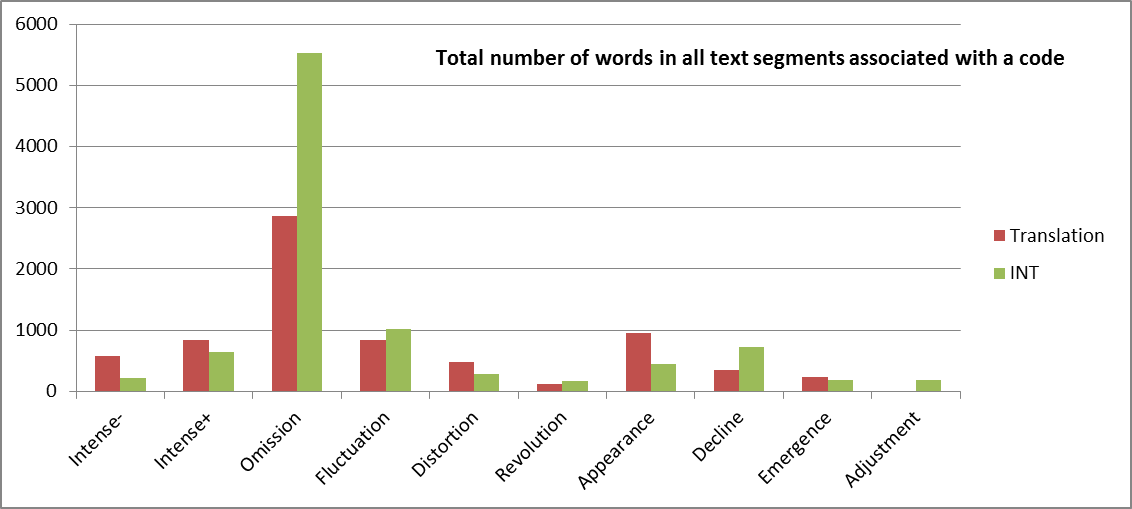
\includegraphics[width=\textwidth]{figures/troqe-marchan/figure4.png}
\caption{Total number of words in all text segments associated with a code}
\label{troqe-marchan:fig:4}
\end{figure}

\begin{figure}
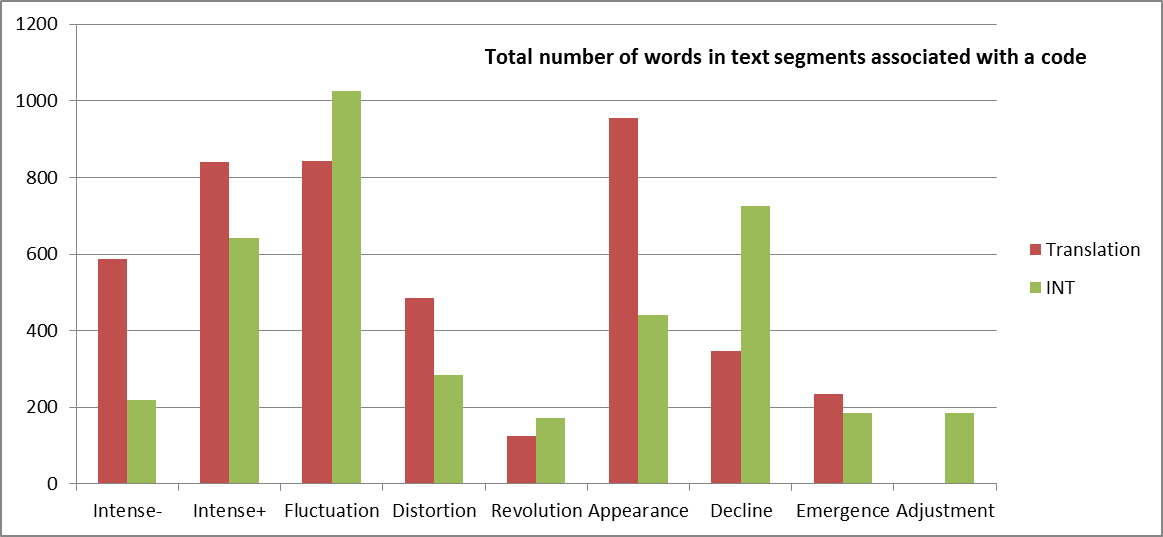
\includegraphics[width=\textwidth]{figures/troqe-marchan/figure5.png}
\caption{Total number of words in text segments associated with a code (except the code \textit{omission})} 
\label{troqe-marchan:fig:5}
\end{figure}

The elision of original segments in the translated texts (\figref{troqe-marchan:fig:4}) is due to the fact that the original articles are chosen and pre-edited, i.e. shortened prior to transmission to the translators. 

Major variations in the edited texts may be due to internal norms, as explained in the interview with one of the deputy directors of the magazine. The main constraint may be space and graphical limitation, which could explain the need to shorten texts. 

\newpage 
Other editorial norms mentioned in Internazionale's \isi{editing} style guide are: 

\begin{itemize}
 \item avoid long sentences and unusual and awkward syntactic constructions;
 \item avoid using special verbal tenses (i.e. pluperfect);
 \item avoid excessive use of pronouns and adjectives, and obsolete words;
 \item maintain, to the greatest possible extent, the specificities of the original language, while ensuring an enjoyable and smoothly readable \ili{Italian}.
\end{itemize}


Of course, these recommendations are not restrictive or binding and editors are free to edit texts as they find appropriate. In fact, as shown by the data, it is true that variations such as Fluctuation and Decline are aimed at avoiding redundancy, long sentences and awkward expressions, but at the same time, downplaying nuances and omitting whole paragraphs does not speak in favour of ``maintaining the specificities of the original'', unless one specifies what is meant by ``specificities''.

Thus, a question naturally emerges: how do editors reshape and transform the translated texts before the editorial board publishes them as \textit{translations} overtly bearing the translators' %
%Can the results be interpreted in terms of \figref{fig:1} and 2? See the two previous paragraphs newly introduces.
names?

\subsection{TAP with Editors}\label{troqe-marchan:sec:b}

A think aloud protocol is a method for gathering data by asking people to perform a task while stating directly what is going on in their heads/minds. This method was first used in psychology studies \citep{Ericsson1993} but was quickly and widely adopted to collect raw data on translation, as demonstrated by the annotated bibliography on TAPs in translation by \citet{Jaaskelainen2002}. TAPs have mainly been collected while subjects perform translation or translation{}-related tasks, i.e. problem solving activities while translating texts from one language to another. Recently, TAPs have also been employed to investigate processes by translation proofreaders and have dealt with issues such as fidelity, time and quality in the \isi{revision} of draft translations \citep{Kunzli2007, Robert2013}. %
%briefly discuss the disadvantages of this method. why is it suitable for tbis study?
Among the biases of the TAP method, there is the difficulty of making sure that the verbalisations actually reflect mental states without distortion, but also the degree of automation performed by subjects experienced in the task which leads to fewer verbalization of conscious mental states in the short term memory compared to subjects who are less experienced and therefore more prone to verbalize a higher amount of information \citep[127]{Ericsson1993}. Notwithstanding these disadvantages, in our case, this method proved to be a useful addition to our tool set: our understanding of translation is enhanced by pooling results derived from the analysis of texts (as provided in \sectref{troqe-marchan:sec:a} of the present study) and responses by those who are involved in the process of making the final products.. In particular, we focus on the responses of the Initiator actant (\figref{troqe-marchan:fig:2}) in order to understand which values (\figref{troqe-marchan:fig:1}) are implemented. 

We have therefore utilized the TAP vocal recording method to collect data while four Internazionale professional editors performed the \isi{editing} of translated texts. 

The test was carried out at Internazionale's offices and was executed in two experiments: 


\begin{enumerate}
 \renewcommand{\labelenumi}{}
 \item Test 1: a trial test, presented as a warm-up exercise, with TAPs collected while editors worked on translations (by translators they usually work with) to be published in the following issue of the magazine;
 \item Test 2: TAPs were collected while editors worked on a translation performed by a \isi{professional translator} with the fictitious brief that the output would be published in the magazine. In Test 2, no layout limitations were given. 
\end{enumerate}

Verbalizations of both experiments were coded according to categories that group together similar information provided in the TAPs referring to particular constraints (editorial norms), to references to the translator's performance, to the readership, or to personal preferences: 

\begin{enumerate}
\renewcommand{\labelenumi}{\roman{enumi}.}%
 \item Editorial constraints: semantic and syntactic preferences for smooth reading, clarity, concision, simplification and space limitation, as well as online research for terminology and fact-checking
 \item Subjectivity
 \item Reference to the translation or translator
 \item Reference to the readership 
\end{enumerate}

In both tests, a large number of verbalizations referred to \textbf{online} \textbf{research}, mostly made to check facts, double check sources, but also to verify terminology in bilingual or monolingual dictionaries. Sometimes the sources were Wikipedia or online news websites; sometimes expressions were googled to see if the expressions translated had a high rate of occurrence in \ili{Italian}. 

\ea \label{troqe-marchan:ex:1}%
\glt verifico\ldots allora \ldots  quindi cerco\ldots  ehm/ manus island detention center\ldots cerco online per verificare se ce ne uno o ce ne sono di più\ldots vediamo\ldots  allora / qui guardo wikipedia in inglese \ldots
\glt I'm checking it\ldots so\ldots I'm looking up\ldots  um / the manus island detention centre\ldots I'm looking online to see if there is one or more than one\ldots  let's see\ldots so / I'm looking up Wikipedia in English...\footnotemark
\z%

\footnotetext{The verbalizations in \ili{Italian} are translated here as clearly and faithfully as possible in order to make them accessible to readers who do not understand \ili{Italian}.}% 

\ea \label{troqe-marchan:ex:2}%
\glt che dal monstero di santa caterina nel Sinai / questa frase la googlo per controllare se in italiano ci sono delle occorrenze e se è un posto consciuto, ecco... dice monastero di santa caterina\ldots
\glt the one about the \textit{monstero di santa caterina nel Sinai} / I'm googling this sentence to check if there are occurrences in \ili{Italian} and if it's a known place, here we go... it says the \textit{monastero di santa caterina}...
\z 

\ea \label{troqe-marchan:ex:3} 
\glt \textit{of petty}\textit{... petty defiance} com'è \textit{defiance}? Insubordinazione? [Cerca \textit{defiance} su un dizionario bilingue online] Di ribellione\ldots  insubordinazione.. / evidentemente c'è una differenza enorme tra questi piccoli atti di ribellione e\ldots
\glt \textit{of petty\ldots } \textit{petty defiance} what is \textit{defiance}? Insubordinazione? [He looks up \textit{defiance} in an online bilingual dictionary] ribellione... insubbordinazione... / \textit{obviously there'}\textit{s a huge difference between these small acts of rebellion and...}
\z 

30.7\% of the coded verbalizations refer to \isi{editing} operations such as changes in the translations motivated by a concern for \textbf{brevity,} \textbf{clarity,} \textbf{simplification} and \textbf{reader engangement}. 

\ea \label{troqe-marchan:ex:4} 
\glt Qui io comincerei a togliere qualcosa perché è una frase molto lunga. (Test1 P2)
\glt Here I'd start cutting something out because the sentence is very long.
\z 

\ea \label{troqe-marchan:ex:5} 
\glt Allora guardo quanto posso tagliare/quanto devo e posso tagliare / Un po' / Per fortuna perché / insomma ci sono un sacco di ripetizioni / e particolari/anche un po' superflui. (Test 1 P3 30.7\%3)
\glt Well, I'm looking at how much I can cut out / what I should and what I can cut out / A bit / Luckily, because / well, there are a lot of repetitions / and details/ that are also a bit unnecessary. 
\z

In \exref{troqe-marchan:ex:4}, one of the editors expresses the need to shorten texts because she thinks the sentence is too long according to editorial constraints, which are not overtly expressed. In Example 5, another editor is verbalizing while having an overall look at the computer screen and assessing that something must be cut out in order to ensure that the text will fit  into the space allowed. 

\ea \label{troqe-marchan:ex:6} 
\glt Sto rileggendo perché secondo me per fare una cosa ben fatta va completamente ristrutturato. (Test2 P1)
\glt I'm rereading it because I think that to do it well, it has to be completely restructured.
\z

\ea \label{troqe-marchan:ex:7} 
\glt È problema dell'articolo e non della traduzione. Pero è un problema. (Test2 P1)
\glt This is a problem with the article, not the translation. But it is a problem.
\z

\ea \label{troqe-marchan:ex:8} 
\glt Io ho fretta\ldots  (sospira) e quindi faccio la cosa più rapida\ldots  / e quindi tolgo un bel pezzone. (Test2 P1)
\glt I'm in a hurry... (sighs) and so I'm doing the fastest thing... / and removing a large chunk.
\z 

In \exref{troqe-marchan:ex:6}, the editor is reading a paragraph and going back and forth between the translation and the original, and he is facing a comprehension problem due to the original text, as verbalized in Example 7. He first tries to solve the problem by doing some online research. Then, having failed to find satisfactory online information, he solves it by completely restructuring the entire paragraph, and by doing away with some unclear information as \exref{troqe-marchan:ex:8} shows time is a constraint factor as well (``I'm in a hurry \ldots~and so I'm doing the fastest thing''). 

\ea \label{troqe-marchan:ex:9} 
\glt il precedente governo federale\ldots  tolgo precedente perché è chiaro è nel 2012 / eh, tolgo \textit{federale} perché per noi che non siamo australiani la distinzione fra governo federale... centrale\ldots  e i governi dei singoli stati / a meno che non si parli dei singoli stati / non interessa\ldots  del governo si capisce. (Test1 P3)
\glt \textit{il precedente governo federale}... I'm removing \textit{precedente} because it's obvious that it's in 2012 / um, I'm removing \textit{federale} because for us, who aren't Australian, the difference between the federal government\ldots the central\ldots  and the state governments / unless we don't speak of state governments / doesn't matter\ldots   \textit{governo} is clear enough.
\z 

\ea \label{troqe-marchan:ex:10} 
\glt \textit{gli agenti antisommossa della G4S sono intervenuti} / allora qui parla della zona Oscar / zona Oscar / guardo l'originale e\ldots  parla di Oscar compound / potrei cercarlo / ma lo tolgo semplicemente perché è un dettaglio che non ci interessa... non è determinante. (Test1 P3)
\glt \textit{gli agenti antisommossa della G4S sono intervenuti} / well here it talks about \textit{zona Oscar} / \textit{zona Oscar} / I'm having a look at the original and\ldots  it says Oscar compound / I could look it up / but I'm removing it simply because it's a detail that isn't of interest to us... it's not relevant.
\z

In \exref{troqe-marchan:ex:10}, one of the editors decides to simplify something by transforming ``previous federal government'' into ``government'' and leaves out some culture specific information because she thinks it is not of any interest to ``us'', while addressing the researcher. Perhaps ``us'' refers to the \ili{Italian} readership, but this is just a hypothesis. Again, in Example 10, she decides to remove a piece of information (\textit{Oscar compound}) that is said not to be of any interest to ``%
%In addition to the discussion of all these verbalizations in detail it would be nice to have some figures or quantifications
us'' (``I could look it up / but I'm removing it simply because it's a detail that isn't of interest to us''). Examples 9 and 10 are significant in terms of showing how far an editor can go with the purpose of rendering the translated text `more readable'.

\ea \label{troqe-marchan:ex:11} 
\glt ehheh.. no, vorrei mettere questa cosa insomma ma in maniera più semplice.. (Test2 P4)
\glt umm\ldots  no, I'd like to put this more simply...
\z 


\ea \label{troqe-marchan:ex:12} 
\glt Una frase lunghissima che vorrei spezzare... allora forse posso trasformarla così.. (Test2 P2)
\glt A very long sentence that I would like to break up... so maybe I could transform it like this...
\z

\exref{troqe-marchan:ex:11} and \exref{troqe-marchan:ex:12} are verbalizations that express the need to reword or change syntactic structures to allow for smooth reading. 

Although 30.7\% of the \isi{editing} is done in the name of editorial needs, 28.8\% of the coded verbalizations refer to rewording, shortening and reshaping based on \textbf{idiosyncrasies,} as expressed in the following verbalizations. In example 13, the editor says he wants to put ``c'è'' (``there is'') in a ``better place'' in the paragraph, but we do not know based on which specific criteria this modification is really better and is really an improvement compared to the translated version. In \exref{troqe-marchan:ex:14}, a personal preference is overtly expressed (``I still \textit{don't like} this sentence\ldots ''), but again we do not know on which basis the editor justifies the likes and dislikes. The idiosyncratic nature of modifications is even more patently manifested in \exref{troqe-marchan:ex:15} and \exref{troqe-marchan:ex:16} (``to me it sounds better''; ``It sounds awful''). 

\ea \label{troqe-marchan:ex:13} 
\glt \textit{C'è evidentemente una differenza enorme} a questo punto mettiamo questo \textit{c'è} in un posto che mi piace di più (sospira).  (Test2 P1)
\glt \textit{C'è evidentemente una differenza enorme} now I'll put this \textit{c'è} in a place that I like better (sighs).
\z 

\ea \label{troqe-marchan:ex:14} 
\glt Continua a non piacermi questa frase perché c'è qualcosa che non va con\ldots  (Test2 P2)
\glt I still don't like this sentence because there is something wrong with \ldots
\z

\ea \label{troqe-marchan:ex:15} 
\glt va beh, io tolgo \textit{possiamo} e scrivo \textit{è possibile} che già dà l'idea della domanda, o comunque / non lo so / a me suona meglio. (Test2 P3)
\glt Ok, I can take away \textit{possiamo} and write \textit{è possibile}, which gives the idea of the question or anyway / I don't know / to me it sounds better.
\z 

\ea \label{troqe-marchan:ex:16} 
\glt \textit{esercizio di associazione di idee}? Ha un bruttissimo suono. (Test2 P4)
\glt \textit{esercizio di associazione di idee}? It sounds awful.
\z 

The TAPs of the first warm-up experiment only show 7.7\% of the coded verbalizations by the editors concerning the \textbf{translators}. However, there is one reference to the translator (\exref{troqe-marchan:ex:17}) by one of the editors in Test 1 that sheds light on the relationship between translators and editors. 

\ea \label{troqe-marchan:ex:17} 
\glt Io non lo leggo continuamente il testo inglese nel momento in cui l'italiano scorre e mi torna/ questo anche perché mi fido del traduttore/ di lui come persona che traduce questa pagina da tanti anni e / si è abbastanza tarata sul tipo di cose che mi piace che ci siano e che non mi piace che ci siano\ldots (Test1 P1)
\glt I don't read the English text all the time when the \ili{Italian} reads smoothly and looks Ok to me / also because I trust the translator / as a person who has translated this page for many years and/ she's quite tuned into the type of things that I do and I don't like...
\z 

The TAPs of Test 2 reveal that when asked to edit a translation by an unknown \isi{professional translator}, editors refer to concepts such as freedom and literality. A total of 15.4\% of the coded verbalizations refer to the translator's performance, the following Examples (18 to 30) are samples of such verbalizations.

\ea \label{troqe-marchan:ex:18} 
\glt Leggo l'inglese perché a questo punto non mi fido veramente più / Il test\ldots  (legge l'inglese) (sospira) / dire \textit{consisteva nel fissare una candela} la fa più facile / di quella che è evidentemente mentre lui qui me la presenta in una maniera più complicata/cioè c'era \textit{indovinare, to work out}, capire come fare a fissare una candela\ldots  (Test2 P1)
\glt I read the English text because at this point I no longer really have any trust / The text\ldots  (reads the English text) (sighs) / to say \textit{consisteva nel fissare una candela} obviously makes things easier / while here he presents it in a more complicated way / that is to say, one must \textit{indovinare}, \textit{to work out}, understand how to fix a candle\ldots 
\z

In \exref{troqe-marchan:ex:18}, one of the editors first expresses general mistrust (the \ili{Italian} verbalization ``\textit{non mi fido veramente più''} is an impersonal form where the direct object is not expressed) then checks the English texts and concludes that the \ili{Italian} translation is simplified compared to the original English. 

\ea \label{troqe-marchan:ex:19} 
\glt Quindi questo lo levo / perché \textit{tra creatività e disonestà} non c'è se le inventato il traduttore.
\glt So I'll leave this out / because there is no \textit{tra creatività e disonestà}; the translator has invented it. 
\z 

\ea \label{troqe-marchan:ex:20} 
\glt Qui è davvero così? Secondo me si è preso troppe libertà il traduttore.
\glt Is it really like this? In my opinion the translator took too many liberties.
\z 

\ea \label{troqe-marchan:ex:21} 
\glt ehm sto cercando\ldots  siccome è molto diversa dalla\ldots  ci sono molte libertà... il traduttore si è preso molte liberta.. sto cercando di capirle fino a che punto posso tollerarle\ldots . e dove devo intervenire per ripristinare\ldots 
\glt umm I'm trying to\ldots  since it's very different from the\ldots  there is too much freedom\ldots  the translator has taken a lot of liberty\ldots  I'm trying to understand to what extent I can accept\ldots  and where should I intervene to restore\ldots  
\z

\ea \label{troqe-marchan:ex:22} 
\glt Io direi più / sarei più\ldots  vicino al testo\ldots  
\glt I would say more / I'd be more... like the text...
\z 

\ea \label{troqe-marchan:ex:23} 
\glt è \textit{la mancanza di onestà}? Cheating lo vogliamo tradurre così? Cheating è più che\ldots  probabilmente guarda se avessi il tempo andrei a guardare in un vocabolario\ldots 
\glt is the \textit{mancanza di onestà} right? \textit{Cheating}, shall we translate it like this? \textit{Cheating} is more likely to be\ldots  probably if I had the time, I'd go and look it up in the dictionary.
\z 

\ea \label{troqe-marchan:ex:24} 
\glt No, qui no, oddio, va totalmente riscritta! / più che scriver / io chiamerei il traduttore e gli direi, senti, me lo rivedi perché non capisco bene com'è fatto.
\glt No, not here... oh God, it has to be completely rewritten! / I wouldn't rewrite it / I'd rather call the translator and say, look, can you check this because I don't really understand it, the way it is.
\z 

\ea \label{troqe-marchan:ex:25} 
\glt No, mi sa che qui è proprio sbagliato l'italiano! Oddio! È totalmente un'altra cosa!
\glt No, I think the \ili{Italian}'s wrong here! Oh my God! It's completely different!
\z
%
%If you provide figures, not all of these verbalizations have to be included in the text.
%The example 18{}-30 are all verbalizations referring to the translator, therefore included into the 15.4\% above mentioned.
In \exref{troqe-marchan:ex:20} to \exref{troqe-marchan:ex:25}, taken from the TAP of the participant 4 shows dissatisfaction with a translation considered to be free and loose compared to the original. There are also some comprehension problems due to information implicit in the original text, as signalled in \exref{troqe-marchan:ex:24}; here, the editor would rather call the translator and ask him/her to review his work or explain what the original means. However, participant 4 decides to rewrite the text himself in a way that is considered closer to the original. Quality assessment is not discussed in this paper, however, it must be said that some mistakes were made while rewording the translation. 

\ea \label{troqe-marchan:ex:26} 
\glt Sì, è una traduzione un po' libera però mi sembra che possa andare bene.
\glt Yeah, it's a bit of a free translation but I think it might be Ok.
\z 

\ea \label{troqe-marchan:ex:27} 
\glt Forse così è più simile a quello che dovrebbe essere.
\glt Maybe this way it's more similar to what it should be.
\z 

\ea \label{troqe-marchan:ex:28} 
\glt Forse lo metterei più simile\ldots  
\glt Maybe I would make this more similar... 
\z 

Verbalizations by participant 2 also refer to the fact that the translation is somewhat free -- though not incorrect -- compared to the original; she seems to be fine with it and changes the translation only a few times to render it closer to the original (\exref{troqe-marchan:ex:27}, \exref{troqe-marchan:ex:28}).

\ea \label{troqe-marchan:ex:29} 
\glt Allora io lascerei più letterale possibile. 
\glt So, I would leave this as literal as possible.
\z 

\ea \label{troqe-marchan:ex:30} 
\glt Allora qui, il traduttore ha tolto la frase\ldots . che però è carina\ldots  eeehhhm A \textit{long\ldots } \textit{it is a long way fr}\textit{om such acts of petty defiance to building a lair inside an extinct volcano and threatening Washington} \textit{from it}\ldots  l'ha riassunta dicendo tra un atto si sfida al governo statunitense come quello perpetrato da Ernst Stavro Blofeld ..   Allora io metterei\ldots 
\glt So, here, the translator has taken this sentence away... which is a nice sentence... uuumm \textit{A long\ldots  it is a long way from such acts of petty defiance to building a lair inside an extinct volcano and threatening Washington from it}\ldots  he's summed it up by saying \textit{tra un atto si sfida al governo statunitense come quello perpetrato da Ernst Stavro Blofeld}\ldots  So I would put\ldots  
\z

Verbalizations 28{}--30 also reveal that participant 3 would like the translator's work be closer to the original and to transform the translation into a more literal version. 

\ea \label{troqe-marchan:ex:31} 
\glt OK qui la traduzione ehm non è letterale / cioè che va bene\ldots  però forse io la cambierei, la metterei un po' più vicino all'originale.
\glt Ok here the translation is umm not literal / that's fine... but maybe I'll change it, I would make it a little more like the original.
\z 

\ea \label{troqe-marchan:ex:32} 
\glt allora, eh, sì, no, qui ha proprio il traduttore ha diciamo riassunto, un po' troppo forse.
\glt well, um, yes, no, here the translator has summed it up a little too much, perhaps.
\z 

\ea \label{troqe-marchan:ex:33} 
\glt L'idea\ldots  è in realtà... del genio malvagio, non è \ldots  \textit{da james bond}... ehhm  l'idea del genio malvagio\ldots  è stata al centro... il genio malvagio, sì metto più aderente all'originale.
\glt The idea\ldots  is actually.... \textit{del genio malvagio}, it isn't... \textit{da james bond}.. ehhm the idea \textit{of genio malvagio}...  was at the centre ... \textit{il genio malvagio}, yes I'll make it closer to the original.
\z

Only 0--9\% of coded verbalizations refer directly to the readership and these are found exclusively in the TAP of participant 1 during the experiment. In the original text, there are many examples of typical English lexical items and oral expressions; in fact, the author discusses the use and evolution of the English language. The translator has decided to keep all the original examples in English and give an \ili{Italian} translation in brackets. Here, the editor reflects on the fact that all the expressions left in English in the \ili{Italian} translation may be too difficult or boring for the readership. 

\ea \label{troqe-marchan:ex:34}
\glt trovo molto faticoso per il lettore / questo pezzo enorme tutto di cose in inglese.
\glt I think this is very hard for the reader / this huge chunk of things, all in English.
\z 

\ea \label{troqe-marchan:ex:35} 
\glt fa fatica a me e quindi penso cha faccia fatica anche al lettore.
\glt it's very hard for me and I think it's hard for the reader as well. 
\z 

\ea \label{troqe-marchan:ex:36} 
\glt e se il lettore non sa l'inglese\ldots  sbatte contro una serie di ostacoli che gli rendono questa cosa molto noiosa\ldots  gliela rendo lo stesso, non ci posso fare nulla... però cerco di rendergliela un po' meno noiosa\ldots  manipolando un po' la cosa.
\glt and if the reader doesn't know English... they come up against obstacles that make this thing very boring... I'll do the same, I can't do anything... but I'll try to make it a bit less boring... by manipulating it a bit.
\z 

\ea \label{troqe-marchan:ex:37} 
\glt Io non voglio che il mio lettore debba fermarsi per fare mente locale su che libro sta parlando\ldots  
\glt I don't want my reader to stop and think about which book is being discussed here...
\z 

Investigation of the think-aloud protocols from four Internazionale editors shows interesting data that would not have been available if only the published articles had been looked at. In fact, participants scrupulously read the translations and originals in order to check the source of information, \isi{monitor} the correspondence between the translations and their originals and then intervene with the internal editorial requirements. Space and layout are the major constraints that account for summarizing and cutting strategies and this can partly explain the high number of omissions found in the text analysis in \sectref{troqe-marchan:sec:a}. Changes in the semantic and syntactic features in the translation, as well as variations in information flow (the order in which events are presented) occur due to the need to render the text smoother, simpler and more %
%Can these results be related to the corpus study in a)?
direct, and these data explain the fact that one of the predominant category found in \sectref{troqe-marchan:sec:a} was none other than Fluctuation. The significant presence of Fluctuations in the text analysis is also explained by the fact that the degree of subjectivity seems to be high, and participants change the translations on the basis of their personal preferences, shaped by their experiences of several years. As discussed above, experience and automation are often considered to bias the results derived from the use of the TAP method (all editors have at least four years of experience). Here, these two factors seem to prompt genuine verbalizations concerning common and widespread editorial practices. It might be interesting to further address the process of translation \isi{editing} from a routinized perspective, i.e. by comparing results derived from TAPs by young editors and TAPs by experienced ones. 

In the verbalizations, the relationship with the translators is clear: editors probably tend to work with the same translators and establish a relationship of trust. This means that translators are trusted as far as fidelity to the source text is concerned, giving editors a free hand in \isi{editing}. In fact, when faced with the work of an unknown \isi{professional translator}, they tend to be suspicious and assume rigid positions demanding more literality and fidelity to the source text. Very few verbalizations take into consideration the readership; editors do not seem to openly consider the reader factor as an argument that might explain their editorial %
%Can the results be interpreted in terms of \figref{fig:1} and 2?
%
choices. In terms of our theoretical background, this part of the study confirms the major role played by the Initiator (\figref{troqe-marchan:fig:1}) in setting the translational agenda with the contractual instructions (what is to be expected by the Translator), the normative environment (what has to be included or omitted), but also the ethical dimension (how to relate to the others, including the author/culture of the source texts as well as the readership/culture of the receiving system). As this part of the study shows, his/her role is preponderant in the making of the final product and thus, in establishing the equivalence/difference profile of the translation compared to the original (\figref{troqe-marchan:fig:2}).

\subsection{Survey among the readership}\label{troqe-marchan:sec:c}

The third part of the study involved an online survey carried out over the course of February 2014. The aim of this survey was to find out what the readership thinks about the magazine's translated articles and their opinion about translation in general. 

Internazionale has 123,000 readers, of whom 33,000 have subscriptions and 90,000 buy copies at a newsstand. 167 readers participated in this study and, although it cannot be said that the population of respondents is representative of Internazionale's readership (the editorial board did not give access to the subscriptions list, which would have ensured appropriate sampling), the data nevertheless reveals interesting patterns. 

\textit{With regard to} \textit{the respondents' socio-demographic profile} -- Gender distribution among respondents is almost equal (48.5\% male, 51.5\% female) and the average age is 32. The majority of the respondents is highly educated (91.2\% attend or have attended university; 42\% have Master's degrees) and most of them live in northern Italy (46.7\%). The majority of the respondents is \ili{Italian} (93.4\%), consider \ili{Italian} to be their mother tongue (92.2\%), claim to know at least one other foreign language (64.1\%) and have travelled outside Italy at least once during  the last year (81.4\%). 

\textit{With regard to the respondents'} \textit{reading habits} -- The majority prefers reading books (93.5\%) and read more than 7 books in the last year (67.6\%); they also read magazines (69.4\%) and a few of them indicate online information and websites as other items they like to read. The majority of respondents read in \ili{Italian} (88.6\%) but also in foreign languages (53.9\%). 

We are in presence of a public of cultivated readers who are familiar with foreign languages, we can therefore expect from them a certain sensitivity or responsiveness concerning the issue of translation.

\textit{With regard to the} \textit{respondents'} \textit{attitude towards the question of} \textit{translation in general} -- 29.3\% of respondents say to be very interested in the issue of translation, 47.9\% of respondents are quite interested and 21.6\% are little or not very %
%What does {\textquotedbl}being interested in the issue of translation{\textquotedbl} mean?
interested. 

Respondents state that the translated articles by Internazionale are easily readable (98.2\%); 93.4\% affirm they convey the thoughts of the authors of the articles written in the %
%Did they compare with the originals?
original language and 88.0\% say translations by Internazionale reflect cultural differences. To test if the participants have ever compared translations with the originals, we asked if it has happened to them to read an article that was poorly translated: 32.3\% say ``sometimes'', 24\% ``never'', while 51.5\% admit that they do not know.

\largerpage
\textit{When asked to give an open definition of what they think an ideal} \textit{translation should} \textit{be} -- 35.3 \% of the coded responses refer to ``fidelity'' and ``absolute respect for the author and the original''; 12\% refer to ``smooth reading'', ``nice and fluid'', ``adapted to the target audience''; 27\% give more elaborate and tempered responses that call for ``fidelity to the source text'' and, at the time, ``adequacy to the \ili{Italian} language and/or to the \ili{Italian} readership''. 25.7\% did not answer this question. 

\textit{When asked} \textit{what a good translation should ideally be} -- Respondents agree (95.3\%) with the fact that, ideally, a good translation must be smoothly readable, it must respect the original in its totality (88\%) as well as the style of the original text (89.8\%) and it has to be comprehensible to the \ili{Italian} readers (79.6\%). When asked if they agree with the statement that ``Ideally a good translation must be suited to the \ili{Italian} context'', respondents are very divided on this point: 53.7\% disagree and 47.3\% agree with the statement. 

\textit{When asked about Interna}\textit{zionale'}\textit{s translations} -- The majority of the respondents (83.9\%) agree with the fact that translations done by the magazine are close to the ideal translation. 

All the respondents (100\%) say that the quality of the translation is important for the quality of the information. However, when asked if they have ever read a bad translation in the magazine, one in every two people say ``I do not know''. This tends to demonstrate -- if the trend is confirmed in a larger population -- that actually readers are not very sensitive to the issue of translation and that they trust the translators. 

The survey is obviously affected by limitations\footnote{We do not address here the issue of the \isi{construction} of public opinion through polling \citep[149--157]{Bourdieu1993}, however with a filter question  we measured respondents’ attitudes towards translation with a filter question and redirected those who were interested in the issue of translation to the more specific questions.}  due to the difficulty in accessing the readership (respondents are volunteers), lack of sampling and a relatively small number of respondents. However, the findings shed some light on the opinions of readers who read a magazine publishing translated material every week. In fact, the majority of respondents say they are interested in the issue of translation and agree with the fact that, in general, translation must adhere %
%In order to assess this issue they have to have access to the originals.
to the original in its totality and respect its style. When asked their opinion on what an ideal translation should be, more than a third clearly refer to fidelity; for less than a third, a good translation must be faithful to the original but also smoothly readable. Perhaps the most interesting result is the fact that an overwhelming majority of respondents say that the quality of the translation is important for the quality of the news but, when asked if they have ever read a bad translation in Internazionale, the majority admits that they do not know. This may be explained by the fact that the respondents believe in the completeness and accuracy of the information given by Internazionale and claim to be satisfied with the magazine's translations, and are therefore not interested in checking the %
%Is it possible to relate these findings to the results in section a) and b)?
%
%Can the results be interpreted in terms of \figref{fig:1} and 2?
%
quality. 

In terms of the semiotic square (\figref{troqe-marchan:fig:2}), undoubtedly the part of the readership we surveyed values equivalence in translation, adherence to the contents and style, and loyalty to the \isi{source language} and culture; with other words, they value the respect of ``otherness''. However, the readers are unfamiliar of the complexity of the Initiator-Translator relation (\figref{troqe-marchan:fig:1}) and therefore unsuspecting of the translational and editorial process texts go through before publication (as in \sectref{troqe-marchan:sec:a} of this study) and unknowing of the backstage and the criteria supporting that process (as in \sectref{troqe-marchan:sec:b}). This unawareness could be seen in terms of trust towards a media outlet that promises to voice unique and fresh perspectives on news -- compared to other \ili{Italian} newspapers and magazines -- which is the credo of Internazionale. Now, this is partly the case, however in terms of degree, in this case, the Initiator of the \isi{translation process} tends to give to the readership what the readership needs (or what is supposedly needed, as demonstrated in \sectref{troqe-marchan:sec:a} and \sectref{troqe-marchan:sec:b}) rather than nourishing it with that otherness (i.e. the fresh and unique perspective of quality foreign news reports) to which the magazine owes its lustre. In other terms, the Initiator feeds the readers in the way and with the information they expect (creating textual products that are profoundly \textit{different} from the original, see \figref{troqe-marchan:fig:1}) rather than changing them in a real confrontation with the other, by promoting products that \textit{adhere} to \isi{source language}/culture (see \figref{troqe-marchan:fig:1}). 

\section{Conclusions} 

This piece of research reveals the complexity of the object of study and the manifold problems arising when it comes to describing the practice of translation. The semiotic approach provides a conceptual framework that allows for the identification of the actants involved in the practice of news translation by Internazionale. 

The analysis of the parallel corpora addresses the enunciative praxis of translation, i.e. the appearance, disappearance and transformation of utterances in the field of discourse. The analysis of translated and edited texts shows that, regardless of language pairs, word or paragraph-cutting strategies and \isi{editing} techniques that tend to harmonize lexicon and privilege directness and simplicity may result in deviations in the argumentative flow. 

The analysis of the think-aloud protocols addresses the motivational drive of the Initiator actant, his/her system of values, expectations regarding the translator's performance and sanctions applied to achieve his/her goals. TAPs with four senior editors confirm that -- in alignment with internal editorial norms -- \isi{editing} made on translations is aimed at smooth reading, concision, simplicity and reader engangement. The degree of subjectivity in rewording and summarizing strategies seems to be high; that also applies to the choice of whether content deserves to be omitted or to reach the reader. ``Journalistic standards'' and ``appeal'' values possibly guide the \isi{editing} process. Interestingly, verbalizations in the think-aloud-protocols reveal that editors perform translation and revision-like activities such as re-reading the original in order to control the accuracy of the translation, consulting monolingual and bilingual dictionaries, and carrying out online research for occurrences of specific expressions in the \isi{target language}. Unsurprisingly, relationships between translators and editors are based on trust and confidence: verbalizations reveal that editors expect the translators to be faithful and adherent to the original. In the present case, this expectation seems to be an implicit contractual requirement, and failure to fulfil it triggers sanction-like interventions by the editor as shown in the verbalizations of Test 2. 

Despite the limitations mentioned above, the survey data provide an interesting picture of the readership's image of the magazine and expectations. Most of the respondents are obviously satisfied with the product they buy and say that translation by Internazionale corresponds to their ideal concept of translation which is, in a more or less nuanced formulation, based on the concept of fidelity. However, most of them trust the magazine to the point that they are not able to say if they have ever read a text which was not well %
%Is a data \isi{triangulation} of a), b) and c) possible? Do the results corroborate each other?
translated. 

The different parts of this study are complementary perspectives that shed light on a complex translational case study and at the same time account for a multilayer analysis -- on both a quantitative and qualitative basis -- of the different instances and practices of meaning generation. In the first part of the study, we derive data from the translated texts and we formulate hypothesies concerning the reasons for such results, which lead us to further investigate the actions and the working environment of the Initiator actant. Actually, in the second part of the study, we see how and why editorial interventions are carried out, and confirm the underlying logic behind our textual results; furthermore, the TAP data allows to enrich the knowledge regarding the social relation between the main actants involved in the translational process, and see how editors position themselves in relation to translators and readership. Our theoretical model, as well as the textual analysis and the TAP study, suggest that the readers' idea of translation does not substantially impact what happens in real terms; this assumption is corroborated by the survey we present in the last part of the study. We believe that, in our study, the \isi{triangulation} of data derived from apparently different objects of study and by means of different methods yields genuine added value and honours the semiotic perspective favouring deeper and broader approach to complex meaning-making and meaning-generating activities.  

\largerpage
Referring to the general definition of translation, as in the semiotic square, it can be said that, despite singularities, the voice of the translator realizes the \textit{equivalence} value (as described in \figref{troqe-marchan:fig:1}): translators do not and are not expected to erase content, alter the narratives and the order in which events are presented in the original, and possibly adhere to the style of the original texts. Because of this attitude, translators seem to endorse the so-called Toury's interference law \citep[276]{Toury1995}, where the make-up of the source text is transferred to the target text; in other words, the more the specificities of this make-up are taken into account the more the target text will show interferences. 

By contrast, the voice of the Initiator tends to realize %
%this is very interesting! Please elaborate!
the value of \textit{difference} (as in \figref{troqe-marchan:fig:1}) since contents are shortened, narratives reshaped, semantic and syntactic features altered in order to conform to specific values, which, in this case, correspond to the magazine's norms and needs. Because of this policy, the Initiator seems to endorse what \citet[268]{Toury1995} calls the law of standardization, where textual relations in the original are often modified in favour of habitual options offered in the receiving system; in other words, actualization of the \textit{difference} value amounts ignoring the specificities of the source text's otherness and showing a high level of resistance to interference, by converting specific source features into the target repertoremes, i.e. signs of an institutionalized systemic repertoire.

Finally, in the studied case, the specific way of telling the readership that ``this is a translation'' causes some other questions to arise, which deserve to be further investigated: what is the degree of covertness of these kinds of practices? What is the translators' degree of awareness and acceptance of these practices? Does translation fulfil its objective if the objective pursued by experienced journalists and editors in the news industry is fulfilled and the public is satisfied? 

\largerpage
\sloppy
\printbibliography[heading=subbibliography,notkeyword=this]
\end{document}

% \textbf{References}
% 
% Bielsa, Esperança. 2007. ``Translation in global news agencies''. \textit{Target} 19:1. 35--55.
% 
% Bielsa, Esperança, Susan Bassnett. (2009). \textit{Translation in Global News}. London and New York: Routledge.
% 
% Bogic, Anna. 2010. Uncovering the Hidden Actors with the Help of Latour: The Making of The Second Sex. MonTI2, 173–192. 
%
% Bourdieu, \citealt{Pierre1993} (1979). ``The Public opinion does not exist''. In: Pierre Bourdieu. \textit{Sociology in Question} (Trans. R. Nice). New Delhi: Sage Publications. 149--157.
% 
% Brook, Jonathan. 2012. The Role of Translation in the Production of International Print News. Three Case Studies in the Language Direction \ili{Spanish} to English. Thesis in Translation Studies, presented at the University of Auckland, New Zealand. 
%
% Brownlie, Siobhan. 2010. ``Representing news from France''. In: Christina Schäffner, Susan Bassnett (eds.) \textit{Political discourse, media and translation}. 32--54.
% 
% Buzelin, Hélène. 2005. ``Unexpected Allies: How Latour's Network Theory Could Complement Bourdieusian Analysis in Translation Studies''. \textit{The} \textit{Translator} 11:2. 193--218.
% 
% Buzelin, Hélène. 2006. ``Independent Publisher in the Networks of Translation''. \textit{TTR} 19:1. 135--173.
% 
% Buzelin, Hélène. 2007a. ``Repenser la traduction à travers le spectre de la coédition''. \textit{META} 52:4. 688--723.
% 
% Buzelin, Hélène. 2007b. ``Translations `in the making'''. In: Wolf, Michaela \& Alexandra Fukari (eds.) \textit{Constructing a Sociology of Translation.} Amsterdam: John Benjamins. 135--169.
% 
% Caimotto, M. Cristina. 2010. ``Translating foreign articles with local implications: a case study''. In: Christina Schäffner, Susan Bassnett (eds). \textit{Political discourse, media and translation}. 76--93.
% 
% Chesterman, Andrew. 1996. ``On Similarity'', \textit{Target} 8, 159-64.
% 
% Chesterman, Andrew, 1997. \textit{Memes of Translation}, Amsterdam, Philadelphia: John Benjamins.
% 
% Ericsson, K. Anders, Herbert A. Simon. 1993. \textit{Protocol Analysis: Verbal Reports as Data} (revised edition). MIT Press, Cambridge, Mass.
% 
% Federici, Federico M. 2010. ``Translations in \ili{Italian} media: the Calipari Case and legitimized texts'' ''. In: Christina Schäffner, Susan Bassnett (eds). \textit{Political discourse, media and translation}. 116--141.
% 
% Fontanille, Jacques. 1989. \textit{Les espaces subjectifs}. Paris: Hachette.
% 
% Fontanille, Jacques. 2003. \textit{Sémiotique du discours}. Limoges: Presses de l'Université de Limoges. [\textit{The Semiotics of Discourse}. Jacques Fontanille. Trans. by Heidi Bostic. New York: Peter Lang Publishing. 2006.]
% 
% Fontanille, Jacques, Claude Zilberberg. 1998. \textit{Tension et signification}. Liège: P. Mardaga. 
% 
% Gorleé Dinda. 1994. \textit{Semiotics and the Problem of Translation: With Special Reference to} \textit{the Semiotics of Charles S. Peirce.} Amsterdam, Atlanta: Rodopi.
% 
% Gouanvic Jean-Marc. 2005. «Objectivation, réflexivité et traduction, Pour une re-lecture bourdieusienne de la traduction~»
% 
% Gouanvic, Jean-Marc. 2005. A Bourdieusian Theory of Translation, or the Coincidence of Practical Instances: Field, `Habitus', Capital and `Illusio'. \textit{The Translator} 11: 2. 147--166
% 
% Greimas, Algirdas J., Joseph Courtés. 1979. \textit{Sémiotique: dictionnaire raisonné de la théorie du langage}. Tome I. Paris: Hachette. [\textit{Semiotics and language: an analytical dictionary}, A. J.  Greimas and J. Courtés. Trans. by Larry Christ, Daniel Patte, James Lee, Edward McMahon II, Gary Phillips, Michael Rengstorf. Bloomington, IN: Indiana University Press. 1982.]
% 
% Greimas, Algirdas J. and François Rastier. 1968. The Interaction of Semiotic Constraints. Yale \ili{French} Studies, No. 41, Game, Play, Literature, 86-105.
%
% Greimas, Algirdas J. 1970. \textit{Du sens: essais sémiotiques}. Paris: Seuil.
% 
% Greimas, Algirdas J. 1983. \textit{Du sens 2: essais sémiotiques}. Paris: Seuil.
% 
% Gumul, Ewa. 2010. ``Explicitating political discourse''. In: Christina Schäffner, Susan Bassnett eds. \textit{Political discourse, media and translation}. 94--115.
% 
% Heilbron, Johan, Gisèle Sapiro. 2007. ``Outline for a Sociology of Translation: Current Issues and Future Prospects.'' In: Michaela Wolf \& Alexandra Fukari (eds.). Constructing a Sociology of Translation, Amsterdam: John Benjamins. 93--107.
% 
% Heilbron, Johan, Gisèle Sapiro. 2002. ``La traduction littéraire, un objet sociologique''. \textit{Actes de la recherche en sciences sociales} 144: 3--6.
% 
% Hernández Guerrero, Mª José. 2011. ``Presencia y utilización de la traducción en la prensa española''. \textit{Meta} 56: 1. 101--118.
% 
% Inghilleri, Moira. 2005. ``The Sociology of Bourdieu and the Construction of the `Object' in Translation and Interpreting Studies''. \textit{The Translator}, 11:2. 125--145.
% 
% Jääskeläinen, Riitta. (2002). Think-aloud protocol studies into translation: An annotated bibliography. Target, 1, 107-136.
%
% Jensen, Devon. 2008. ``Credibility''. In: Lisa M. Given (ed.) \textit{The SAGE Encyclopedia of Qualitative Research Methods}. Vol. 1-2. Thousand Oaks, Calif. : Sage Publications. 
% 
% Leech, L. Nancy. 2007.  ``An Array of Qualitative Data Analysis Tools: A Call for Data Analysis Triangulation'' \textit{School Psychology Quarterly}. 22/4. 557--584
% 
% Munday, Jeremy. 2007. ``Translation and Ideology.'' \textit{The Translator}. 13:2. 195--217.
% 
% Nida A. Eugene. 2004. ``Similar but Different.'' In S. Arduini and R. Hodgson, eds. \textit{Similarity and Difference in Translation: Proceedings of the International Conference on Similarity and Translation}. Rimini: Guaraldi. 15--24.
% 
% Petrilli, Susan. 1992. ``Translation, semiotics, and ideology.'' \textit{TTR} 5, 1. 233--264.
% 
% Pym Anthony. 2004. The Moving Text Localization, Translation, and Distribution. Amsterdam, Philadelphia : J. Benjamins.
%
% 
% Robert, Isabelle S. 2013. Translation Revision: Does The Revision Procedure Matter?  In M. Bartlomiejczyk, R. Meylaerts, S. Vandepitte et C. Way, dir. Treks and Tracks in Translation Studies. Amsterdam/Philadelphie, John Benjamins, 87-102.
%
%
% Sapiro, Gisèle. 2008. ``Translation and the field of publishing A commentary on Pierre Bourdieu's ``A conservative revolution in publishing''
%  
% Schäffner, Christina, Susan Bassnett (eds). 2010. \textit{Political discourse, media and translation}. Newcastle: Cambridge Scholars Publishing.
% 
% Stecconi, Ubaldo. 2004. ``Interpretive semiotics and translation theory: The semiotic conditions to translation.'' \textit{Semiotica} 150, 1/4. 471--489.
% 
% Stetting, Karen. 1989. ``Transediting -- A new term for coping with the grey area between \isi{editing} and translating''. ed. G. Cale. \textit{Proceedings from the fourth Nordic conference for English studies}. University of Copenhagen. 371--382.
% 
% Tapia Sasot de Coffey, Maria Josefina. 1992. ``La traducción en los medios de prensa.'' \textit{Babel} 38:1. 59--63.
% 
% Toury, Guideon. 1995. \textit{Descriptive Translation Studies and Beyond}. Amsterdam, Philadelphia. John Benjamins.
% 
% Troqe, Rovena. 2014a. \textit{Traduttolgia e semiotica generativa}\textit{: per un nuovo approccio interdisciplinare}. Peter Lang: Bern. 
% 
% Troqe, Rovena. 2014b. ``On the concept of translation: A perspective based on Greimassian semiotics.'' \textit{Semiotica} 204. 33--59. DOI:~\href{http://dx.doi.org/10.1515/sem-2014-0045}{10.1515/sem-2014-0045},
% 
% Tsai, Claire. 2010. ``News translator as reporter''. In: Christina Schäffner, Susan Bassnett (eds). \textit{Political discourse, media and translation}. 178--197.
% 
% 
% \begin{verbatim}%%move bib entries to  localbibliography.bib
% \end{verbatim} 
